\IEEEPARstart{F}{ace} recognition is a part of biometrics, as well as fingerprints, analysis of hand geometry, iris, retina and voice.
The main application field of biometrics is the access control. It provides solutions safe, cheap, simple and effective.
But in recent years, emerging biometrics in civil matters, for recreational, social and practical purposes.

\subsection{For the access control}

There are two main areas in biometrics : identification and verification.

\paragraph{In the verification or authentication} the biometric system asks the user's identity and tries to answer the question, "Is this person X? ". In an application of the verification system is reliant on biometric information from the user, and compares the data obtained from the characteristic information input with the recorded data corresponding to the asserted identity, it is a one to one comparison (1:1).

The system will find or not find a matching between the two. Verification is commonly used in applications of access control and payment authentication. Biometrics offers many advantages over existing methods of personal authentication such as keys, identification numbers (ID), passwords and swipe cards. Indeed it provided more security and convenience that generates enormous economic benefits and fills the security vulnerabilities of passwords, especially with the current facilities to perform attacks and make cracking.

Thus, these applications are used to identify a large number of people in real time. They are fast and accurate because the reference image has a good quality and image control is taken from the front in optimal conditions.

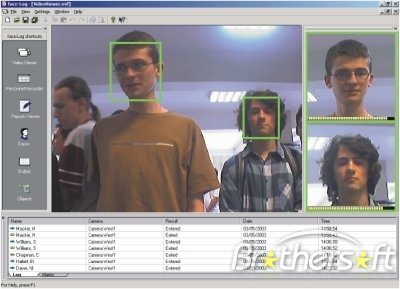
\includegraphics[width=\linewidth]{img/face_recognition_civil}
~\\
Exemples of applications : Passport verification at the airport, windows logon, access to a secure area 

\paragraph{With the identification or recognition} the biometric system asks and attempts to answer the question, "Who is the person X? ". In an identification application, the biometric device requested a biometric information and compares it with every piece of information stored in the database is a comparison to multi (1: N). The object identification applications is to identify criminals and terrorists using the surveillance data.

However, the identification of a suspect filmed by a CCTV camera where conditions are less optimal.
The image is often of poor quality, not always face, facial expression is not neutral, the brightness is different reference pictures.
Again, this time the comparison is not with a single image but with a whole database. The work to be done quickly became much more consistent.

The table~\cite{NPIA} below shows the similarity between the fingerprints searching and the face recognition.

~\\
\begin{tabular}{|p{0.28\linewidth}|p{0.28\linewidth}|p{0.28\linewidth}|}
\hline
\textbf{Fingerprints searching}&\textbf{Face Recognition}&\textbf{Capability}\\
\hline
Ten print to Ten print searching&Mugshot to Mugshot&Identification of an Live Image to Mugshot individual in custody\\
\hline
Ten print to Mark searching&Mugshot to CCTV image&Linking known individuals to unsolved crimes\\
\hline
Mark to Ten print searching&CCTV image to Mugshot&Identifying suspects from forensic evidence at crime scenes\\
\hline
Mark to Mark&CCTV images from multiple cameras&Linking unsolved crimes together\\
\hline
\end{tabular}

~\\
\subsubsection{What are the difficulties ? }
\subsubsection{How does it work ? }

\subsection{Face expression recognition}

